\newpage
\begin{center}
    \rule{\linewidth}{0.2 mm} \\[0.4 cm]
	{ \huge \bfseries Mini-Projects A \& B}\\
	\huge Terrarium Logger
	\rule{\linewidth}{0.2 mm} \\[1.5 cm]
	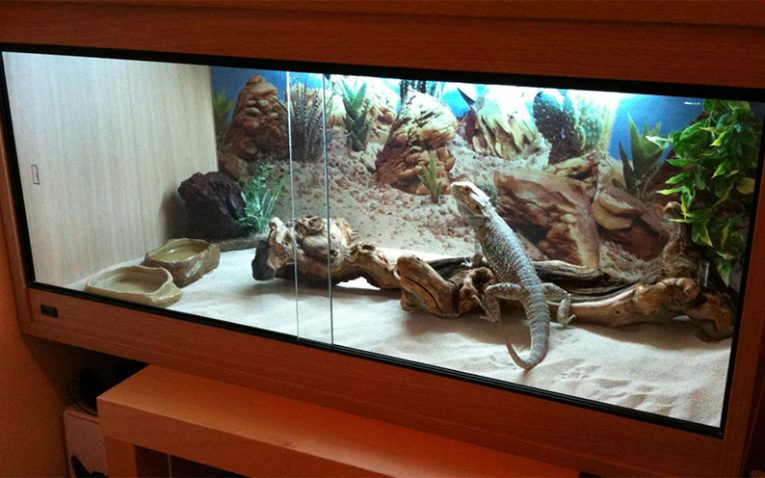
\includegraphics[scale = 0.5]{Figures/terrarium.jpg}\\[1 cm]
	\textsc{\Large EEE3096S}\\[0.5 cm]
	\textsc{\large Embedded Systems II}\\[0.5 cm]
	\textsc{\LARGE University of Cape Town}\\[0.5 cm]
\end{center}
\newpage
\chapter{The Terrarium Mini-logger}
\section{Overview}
The mini-project is a chance for you to use what you have learnt in this course and test your problem-solving skills. The projects use everything learnt in the previous practicals - so here's to hoping that you paid attention and remembered those! All students need to do Mini-Project A. Only CS students (EEE3095S students) need to do Mini-Project B.

\subsection{Scenario}
Your uncle has heard of you achieving great things in an embedded systems course at university. He approaches you and requests your assistance in building an environment logger for his terrarium to assist with taking care of his pet bearded dragon. As they are ridiculously adorable (bearded dragons, not uncles) - you agree to assist.

\begin{figure}[H]
\centering
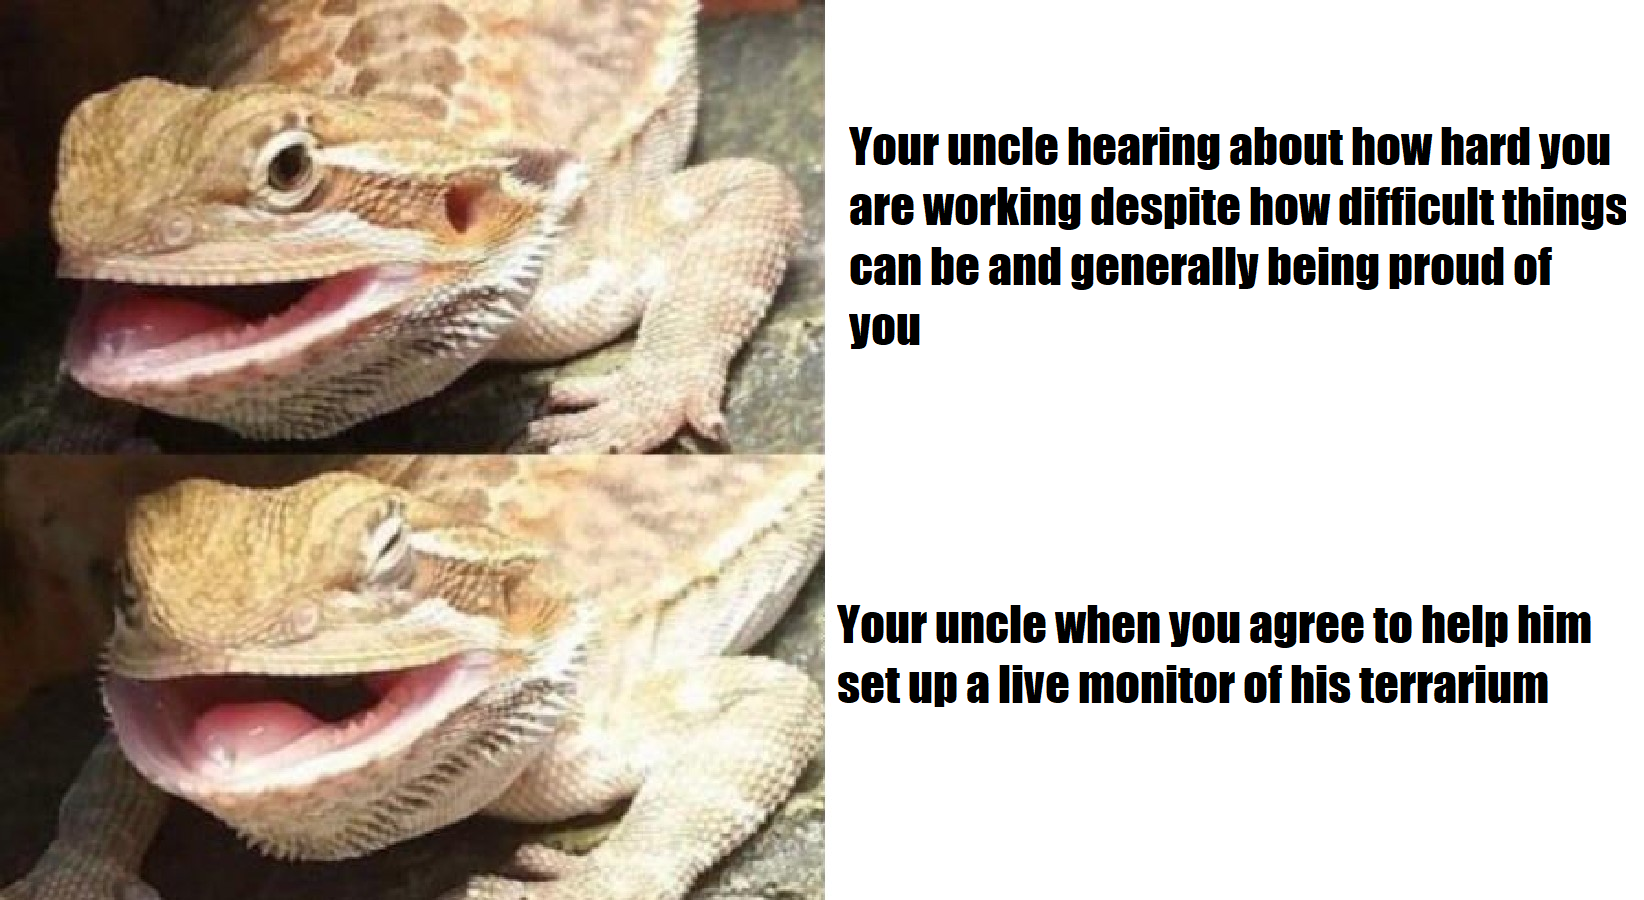
\includegraphics[width=0.7\columnwidth]{Figures/uncledragon.png}
\caption{You can read more about this adorable creature \href{https://knowyourmeme.com/memes/butter-the-bearded-dragon}{here}}
\label{ButterDragon}
\end{figure}

Your uncle needs to monitor temperature and light levels at varying intervals, which needs to be adjusted by a button press. He also wants to enable and disable logging by pressing a second button. Your uncle has a spare system which they can use to log into the Pi remotely and monitor console output, which he lists as one of the requirements. However, they wish to also monitor the terrarium remotely when they are not there. Their son, who plays with Arduinos, has spoken a lot about \href{https://blynk.io/}{Blynk} for IoT devices. You decide to look into these options for remote monitoring. 

The following requests were also made:
\begin{itemize}
    \item the most recent 20 samples are stored on an EEPROM chip as backup, in the case that internet access is lost.
\end{itemize}


\subsection{Basic Details}
Your objective for Mini-Project A environment logger. Mini-Project B is an add-on to Mini-Project A which involves minimal work to extend the functionality of the monitoring system. If you are in a group with both CS and EE members, you can both work together on Mini-Project A. For Mini-Project B, CS students can chose to work alone or partner up with another CS student to form new groups of 2.

Generally speaking, an environment logger interacts with the world around it by measuring various factors from GPS location to air pollution. While a single sensor is useful to monitor a single location, many can be scattered around a broader area to monitor that area as well as any patterns emerging in that broader area. This data can be used to track changes over time to forecast effects or make inferences between locations and how they might affect each other. In these mini-projects there is not much data to track and there aren't many potential effects to forecast, though the principles remains the same.

Project A and B differ in how that data is presented to end users. Project A is simply accessed through a terminal. Project B will add reporting data to Blynk, an app that can be installed on smartphones. The environment logger can also be controlled via the Blynk app.

\textbf{NOTE: FOR EACH SUBMISSION, BOTH STUDENTS NEED TO INCLUDE A SIGNED PLAGIARISM DECLARATION AT THE END OF THE SUBMISSION, WITH THE SUBMISSION AND BOTH PLAGIARISM DECLARATIONS IN A SINGLE PDF. THE FORM CAN BE FOUND AT THE END OF THIS MANUAL.}

\chapter{Mini-Project A}
\label{sec:ProjA}
This project examines ELO5.2, which requires the student to develop a representative embedded system. It requires hardware/software interfacing, so an ADC is sampled by software, and processing operations are applied to read the data. 

\section{Project Requirements}
The Project is split into Milestones in order to help you plan time and ensure you aren't overburdened with work a few days before the final deadline. Dates for submission will be put on Vula. The milestones are as follows:
\begin{enumerate}
    \renewcommand{\theenumi}{\Alph{enumi}}
    \item Planning and System Design\\
    For this milestone we expect to see the following:
    \begin{itemize}
        \item A Gantt Chart indicating your planned activities with the project
        \item A circuit diagram for the system
        \item A choice on how you plan to approach the project (e.g. Spiral, waterfall, etc.) as well as a justification as why
        \item A flowchart detailing how the system operates
    \end{itemize}
    \item Code and Report\\
    The final hand in will be the report and your code submission. Details on these can be found in the marking guides.
\end{enumerate}

\section{Outcomes}
In addition to creating a working system, you will learn about the following in this project:
\begin{itemize}
    \item Technical outcomes
    \begin{itemize}
        \item ADC - \href{https://cdn-shop.adafruit.com/datasheets/MCP3008.pdf}{MCP3008}
        \item Temperature sensor - \href{http://ww1.microchip.com/downloads/en/devicedoc/20001942g.pdf}{MCP9700A}
        
    \end{itemize}
    \item Other outcomes
    \begin{itemize}
        \item Team Work
        \item Design methodologies, such as the Waterfall, Spiral and V Models.
        \item Planning and time management
    \end{itemize}
    
    
\end{itemize}

\section{Deliverables}
At the end of this project, you must:
\begin{itemize}
    \item Submit all milestones
    \item For information on the marks and what sections to cover, refer to the marking guide in Section \ref{sec:ProjAMarks}
\end{itemize}

\section{System Overview}
Figure \ref{fig:SystemOverview} shows the system overview for the mini-project.
\begin{figure}[H]
\centering
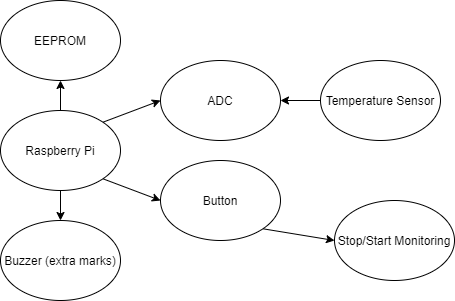
\includegraphics[width=0.6\columnwidth]{Figures/2020-SystemOverview-A}
\caption{Components of Mini-Project A}
\label{fig:SystemOverview}
\end{figure}

\section{Hardware requirements}
You will need to build your designed circuit on a breadboard and demonstrate it in the video you create.

\section{Software requirements}
You need to do the following:
\begin{itemize}
    \item Set up the EEPROM. 
    \item Create a thread for reading from the ADC. The value read from the temperature sensor needs to be converted to degrees Celsius. See the datasheet (linked above) for the formula.
    \item Create interrupts for all the button functionality (don't forget to debounce your inputs)
    \item Create an output signal to trigger the buzzer (bonus marks)
    \item In the main() loop, print values to the screen as described in Section \ref{sec:ProjDescription}
\end{itemize}

\section{Description}
\label{sec:ProjDescription}
\begin{itemize}
    \item By default, the system continuously monitors the sensors every 5s using this format:
    \begin{table}[H]
    \centering
    \begin{tabular}{|l|l|l|l|}
    \hline
    Time     & Sys Timer & Temp  &  Buzzer  \\ \hline
    10:17:15 & 00:00:00  & 25 C  & *        \\ \hline
    10:17:20 & 00:00:05  & 25 C  &          \\ \hline
    10:17:25 & 00:00:10  & 25 C  &          \\ \hline
    10:17:30 & 00:00:15  & 25 C  &          \\ \hline
    10:17:35 & 00:00:20  & 25 C  &          \\ \hline
    10:17:35 & 00:00:20  & 25 C  & *        \\ \hline
    \end{tabular}
    \end{table}
    \item The stop switch stops or starts the monitoring of the sensors. The system timer is not affected by this functionality. The screen must also be cleared when logging is stopped, and a message printed to display to inform the user that the logging has stopped.
\end{itemize}

\section{Marking Guide}
\label{sec:ProjAMarks}
\begin{longtable}[c]{|l|l|}
\caption{Project A marking Guide}
\label{tbl:ProjAMarks}
\\\hline
\textbf{Heading} & \textbf{Report} \\ \hline
\endfirsthead
%
\endhead
%
Introduction & \begin{tabular}[c]{@{}l@{}}Provide a short introduction ($\sim \frac{1}{2}$ page) to your project explaining your main\\ design choices and how the report has been structured \textbf{{[}15 marks{]}}\end{tabular} \\ \hline
Requirements & \begin{tabular}[c]{@{}l@{}}The requirements section should provide a refined UML Use Case\\ diagram of the system, according to your implementation, and any\\ accompanying text that is needed to clarify the requirements.\\ Highlight any departures or additions that you may have made compared to\\ the original project description given in this document. \textbf{{[}15 marks{]}}\end{tabular}  \\ \hline
\begin{tabular}[c]{@{}l@{}}Specification \\ and Design\end{tabular} & \begin{tabular}[c]{@{}l@{}}This section should provide a UML State Chart describing the main\\ operation. Add a UML class or deployment diagram (or other suitable\\ diagram) to indicate the structuring of your implementation (e.g. code\\ modules/classes you may be using). You don’t need to provide fine detail of\\ the system, the diagram(s) can be e.g. at the level of functions. You should\\also include a circuit diagram \textbf{{[}20 marks{]}}\end{tabular}  \\ \hline
Implementation & \begin{tabular}[c]{@{}l@{}}This section should give some snippets of important code and explanations for\\ this (or referring to particular functions in code files). The point here\\ is elaborating any parts of the State Chart that are not so straightforward\\ to turn into code. \textbf{{[}20 marks{]}}\end{tabular} \\ \hline
\begin{tabular}[c]{@{}l@{}}Validation and\\ Performance\end{tabular} & \begin{tabular}[c]{@{}l@{}}Provide at least a paragraph or two explaining the performance of the\\ system. A snapshot could be included and you could show test cases where\\ you have tested that the system works reliably (e.g. using a powersupply to set \\ the value given to the ADC). \textbf{{[}20} \textbf{marks{]}}\end{tabular} \\ \hline
Conclusion & \begin{tabular}[c]{@{}l@{}}Give a summary of the extent that the system was found to be successful.\\ Discuss if you think that a system working in this way might be\\ considered a potentially useful product. \textbf{{[}10 marks{]}}\end{tabular}  \\ \hline
References & Provide a few references if relevant.  \\ \hline
Total & 100 \\ \hline
\end{longtable}
\chapter{Mini-Project B}
This project is for CS students only.\\

\section{Scenario}
Your uncle appreciates the work you have done developing a rough prototype. Because you did such a good job of developing the base system, your uncle has asked you to develop a means of a system where they can access their data remotely. You decide to do this as simply as possible, making use of an application called \href{https://blynk.io/}{Blynk}.



\subsection{Overview}
Essentially, this is a repeat of the first project, but adds a button to change the interval reading and makes the data accessible through Blynk.

\subsection{Deliverables}
At the end of this practical, you must
\begin{itemize}
    \item Submit a short write up. See the marking guide in section \ref{sec:ProjBMarks}
\end{itemize}

\subsection{Hardware Required}
The hardware from mini-project A and an additional button.

\subsubsection{Software Requirements}
\begin{itemize}
    \item You need to add Blynk.
    \item You need to add functionality for changing the reading interval between 2, 5 and 10 seconds.
\end{itemize}

\begin{multicols}{2}
Figure \ref{fig:blynkexample} shows an example of what the app you create in Blynk might look like. This is the example from last year's project, but you can see there's a terminal for accessing the output of the print statements and a space for values as read from the ADC. Last year's project also had an alarm, which is not a feature in this year's project so you need not include one. There are various widgets in Blynk. It's suggested you play with your energy budget to develop the most intuitive and aesthetically pleasing design possible.
\vfill\null
\columnbreak
\begin{figure}[H]
\centering
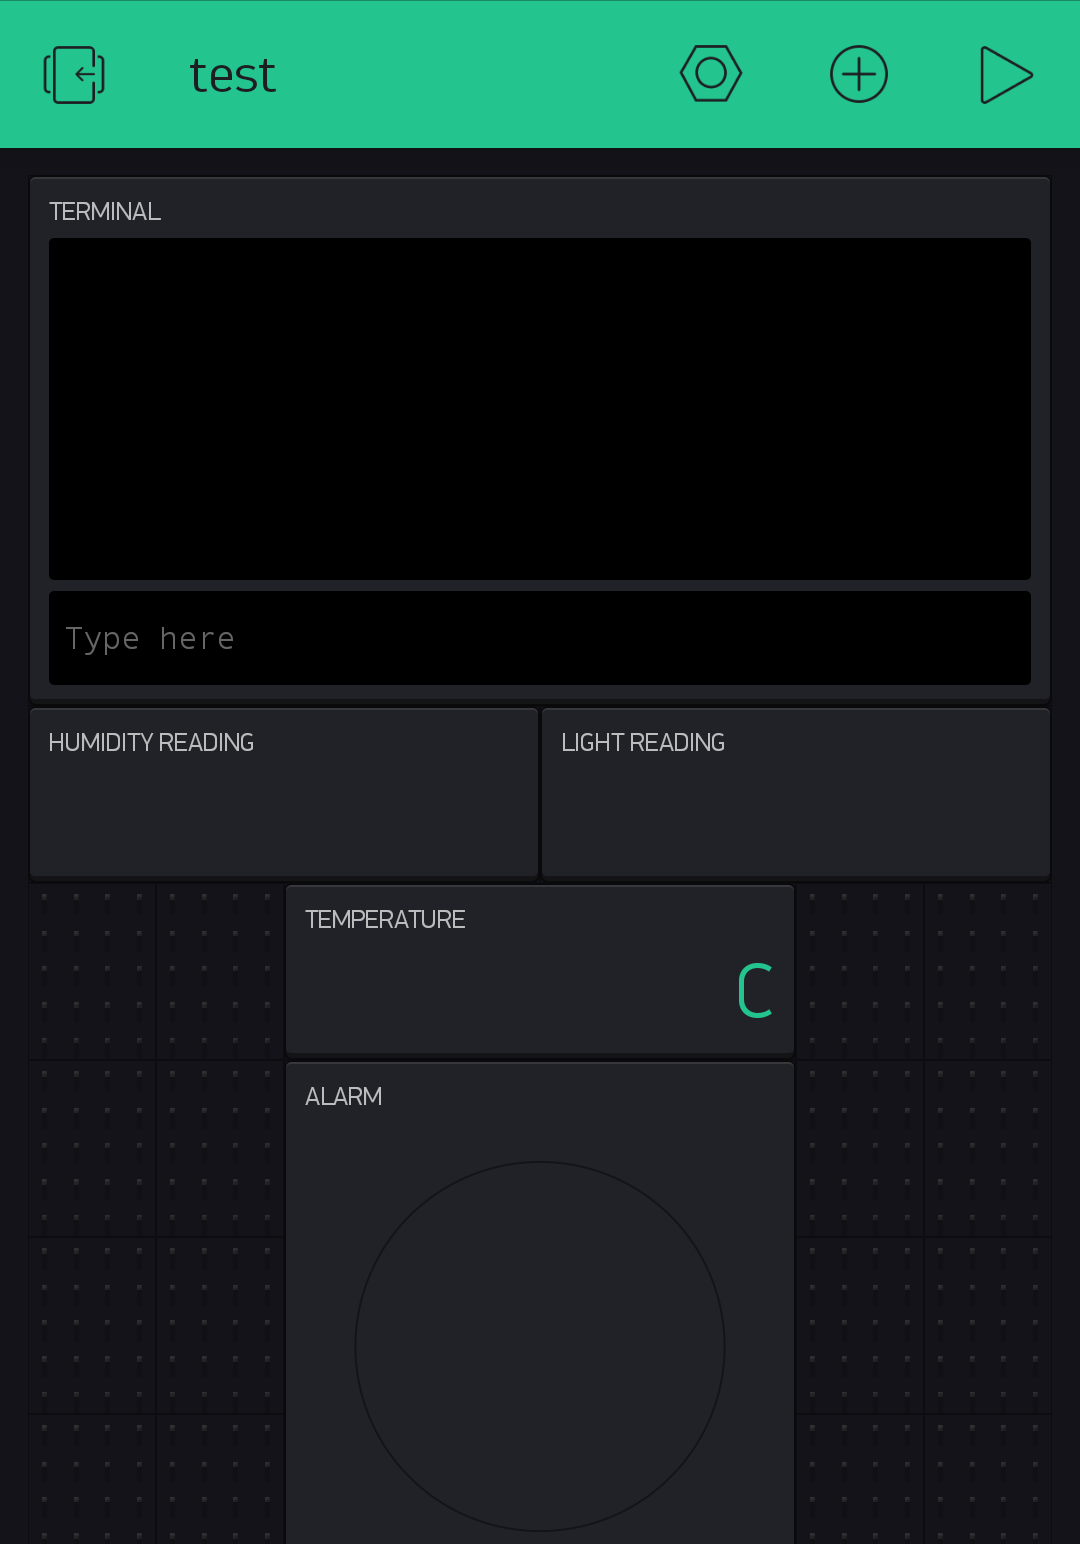
\includegraphics[width=0.75\columnwidth]{Figures/blynkexample}
\caption{Example Blynk Project}
\label{fig:blynkexample}
\end{figure}
\end{multicols}

\subsection{Marking Guide}
\label{sec:ProjBMarks}
\begin{table}[H]
\centering
\caption{The Write Up Format For mini-project B}
\label{tbl:ProjBMarks}
\begin{tabular}{|l|l|l|}
\hline
\textbf{Section of Report} & \textbf{Description} & \textbf{Marks} \\ \hline
\textbf{Introduction} & An introduction to what's new in this project & 10 \\ \hline
\textbf{Design} & \begin{tabular}[c]{@{}l@{}}Design of the system. Design of the server. \\ Talk about the stack used for development. \\ Include UML and block diagrams, and \\ mention any hardware/software\\ interfacing issues.\end{tabular} & 30 \\ \hline
\textbf{\begin{tabular}[c]{@{}l@{}}Implementation/\\ Build Proces\end{tabular}} & \begin{tabular}[c]{@{}l@{}}Some code snippets and steps in building \\ the device and server.Can think of this as a\\ simple methodology.\end{tabular} & 15 \\ \hline
\textbf{Instructions for use} & \begin{tabular}[c]{@{}l@{}}How to operate the system. You should \\ include some screenshots and photos.\end{tabular} & 15 \\ \hline
\textbf{Testing/Results} & \begin{tabular}[c]{@{}l@{}}How did you ensure your system works? \\ What did you do to test the functionality, \\ and what were the results? You can include\\ screenshots or photos, but you need to talk \\ about them (it's not enough to just have a \\ photo).\end{tabular} & 20 \\ \hline
\textbf{Conclusions} & \begin{tabular}[c]{@{}l@{}}How well did your system work? Did you \\ achieve the objectives? What could you do \\ to improve the system?\end{tabular} & 10 \\ \hline
\textbf{TOTAL} &  & \textbf{100} \\ \hline
\end{tabular}%
\end{table}


\chapter{Acknowledgements}
\begin{enumerate}
    \item Image use \href{https://onlineplantsindubai.weebly.com/uploads/1/0/9/0/109064913/air-plants-terrarium-as-bearded-dragon-terrarium_1_orig.jpg}{onlineplantsindubai.weebly.com}
    \item The meme template used in Figure \ref{ButterDragon} is of Butter the bearded dragon, which is accessible through a Google search
\end{enumerate}

\newpage

\textbf{Declaration of non-plagiarism}

\begin{itemize}
    \item I know that plagiarism is wrong. Plagiarism is to use another’s work and pretend that it is one’s own.
    \item I have used the \rule{4cm}{1pt} convention for citation and referencing. Each contribution to, and quotation in, this essay/report/project/submission from the work(s) of other people has been attributed, and has been cited and referenced.
    \item This essay/report/project/submission is my own work.

    \item I have not allowed, and will not allow, anyone to copy my work with the intention of passing it off as his or her own work. 

\end{itemize}

 

Name \rule{4cm}{1pt}  Student Number \rule{4cm}{1pt}

 

Signature \rule{4cm}{1pt}     Date \rule{4cm}{1pt}

 



